% Options for packages loaded elsewhere
\PassOptionsToPackage{unicode}{hyperref}
\PassOptionsToPackage{hyphens}{url}
\PassOptionsToPackage{dvipsnames,svgnames,x11names}{xcolor}
%
\documentclass[
  letterpaper,
  DIV=11,
  numbers=noendperiod]{scrartcl}

\usepackage{amsmath,amssymb}
\usepackage{iftex}
\ifPDFTeX
  \usepackage[T1]{fontenc}
  \usepackage[utf8]{inputenc}
  \usepackage{textcomp} % provide euro and other symbols
\else % if luatex or xetex
  \usepackage{unicode-math}
  \defaultfontfeatures{Scale=MatchLowercase}
  \defaultfontfeatures[\rmfamily]{Ligatures=TeX,Scale=1}
\fi
\usepackage{lmodern}
\ifPDFTeX\else  
    % xetex/luatex font selection
\fi
% Use upquote if available, for straight quotes in verbatim environments
\IfFileExists{upquote.sty}{\usepackage{upquote}}{}
\IfFileExists{microtype.sty}{% use microtype if available
  \usepackage[]{microtype}
  \UseMicrotypeSet[protrusion]{basicmath} % disable protrusion for tt fonts
}{}
\makeatletter
\@ifundefined{KOMAClassName}{% if non-KOMA class
  \IfFileExists{parskip.sty}{%
    \usepackage{parskip}
  }{% else
    \setlength{\parindent}{0pt}
    \setlength{\parskip}{6pt plus 2pt minus 1pt}}
}{% if KOMA class
  \KOMAoptions{parskip=half}}
\makeatother
\usepackage{xcolor}
\setlength{\emergencystretch}{3em} % prevent overfull lines
\setcounter{secnumdepth}{-\maxdimen} % remove section numbering
% Make \paragraph and \subparagraph free-standing
\ifx\paragraph\undefined\else
  \let\oldparagraph\paragraph
  \renewcommand{\paragraph}[1]{\oldparagraph{#1}\mbox{}}
\fi
\ifx\subparagraph\undefined\else
  \let\oldsubparagraph\subparagraph
  \renewcommand{\subparagraph}[1]{\oldsubparagraph{#1}\mbox{}}
\fi


\providecommand{\tightlist}{%
  \setlength{\itemsep}{0pt}\setlength{\parskip}{0pt}}\usepackage{longtable,booktabs,array}
\usepackage{calc} % for calculating minipage widths
% Correct order of tables after \paragraph or \subparagraph
\usepackage{etoolbox}
\makeatletter
\patchcmd\longtable{\par}{\if@noskipsec\mbox{}\fi\par}{}{}
\makeatother
% Allow footnotes in longtable head/foot
\IfFileExists{footnotehyper.sty}{\usepackage{footnotehyper}}{\usepackage{footnote}}
\makesavenoteenv{longtable}
\usepackage{graphicx}
\makeatletter
\def\maxwidth{\ifdim\Gin@nat@width>\linewidth\linewidth\else\Gin@nat@width\fi}
\def\maxheight{\ifdim\Gin@nat@height>\textheight\textheight\else\Gin@nat@height\fi}
\makeatother
% Scale images if necessary, so that they will not overflow the page
% margins by default, and it is still possible to overwrite the defaults
% using explicit options in \includegraphics[width, height, ...]{}
\setkeys{Gin}{width=\maxwidth,height=\maxheight,keepaspectratio}
% Set default figure placement to htbp
\makeatletter
\def\fps@figure{htbp}
\makeatother

\usepackage{booktabs}
\usepackage{longtable}
\usepackage{array}
\usepackage{multirow}
\usepackage{wrapfig}
\usepackage{float}
\usepackage{colortbl}
\usepackage{pdflscape}
\usepackage{tabu}
\usepackage{threeparttable}
\usepackage{threeparttablex}
\usepackage[normalem]{ulem}
\usepackage{makecell}
\usepackage{xcolor}
\KOMAoption{captions}{tableheading}
\makeatletter
\@ifpackageloaded{caption}{}{\usepackage{caption}}
\AtBeginDocument{%
\ifdefined\contentsname
  \renewcommand*\contentsname{Table of contents}
\else
  \newcommand\contentsname{Table of contents}
\fi
\ifdefined\listfigurename
  \renewcommand*\listfigurename{List of Figures}
\else
  \newcommand\listfigurename{List of Figures}
\fi
\ifdefined\listtablename
  \renewcommand*\listtablename{List of Tables}
\else
  \newcommand\listtablename{List of Tables}
\fi
\ifdefined\figurename
  \renewcommand*\figurename{Figure}
\else
  \newcommand\figurename{Figure}
\fi
\ifdefined\tablename
  \renewcommand*\tablename{Table}
\else
  \newcommand\tablename{Table}
\fi
}
\@ifpackageloaded{float}{}{\usepackage{float}}
\floatstyle{ruled}
\@ifundefined{c@chapter}{\newfloat{codelisting}{h}{lop}}{\newfloat{codelisting}{h}{lop}[chapter]}
\floatname{codelisting}{Listing}
\newcommand*\listoflistings{\listof{codelisting}{List of Listings}}
\makeatother
\makeatletter
\makeatother
\makeatletter
\@ifpackageloaded{caption}{}{\usepackage{caption}}
\@ifpackageloaded{subcaption}{}{\usepackage{subcaption}}
\makeatother
\ifLuaTeX
  \usepackage{selnolig}  % disable illegal ligatures
\fi
\usepackage{bookmark}

\IfFileExists{xurl.sty}{\usepackage{xurl}}{} % add URL line breaks if available
\urlstyle{same} % disable monospaced font for URLs
\hypersetup{
  pdftitle={Lov utan lov},
  colorlinks=true,
  linkcolor={blue},
  filecolor={Maroon},
  citecolor={Blue},
  urlcolor={Blue},
  pdfcreator={LaTeX via pandoc}}

\title{Lov utan lov}
\author{}
\date{}

\begin{document}
\maketitle

Vi kan börja med att analysera hur frånvaron fördelas över våra skolor,
särskilt andelen beviljad ledighet. Råå södra skola har den högsta
andelen beviljad ledighet, där 1,2\% av all lektionstid förloras på
grund av godkänd ledighet. I andra änden av spektrat hittar vi Gantofta,
där endast 0,1\% av lektionstiden missas av samma anledning. När
skolorna sorteras efter andelen beviljad ledighet framträder en tydlig
trend: skolor med resursstarka föräldrar tenderar att ligga till
vänster, medan de med mindre resursstarka föräldrar återfinns till
höger. Även om det finns en del undantag. En djupare analys av
socioekonomiska faktorer kan ge ytterligare insikter i hur dessa
påverkar frånvaromönstren.

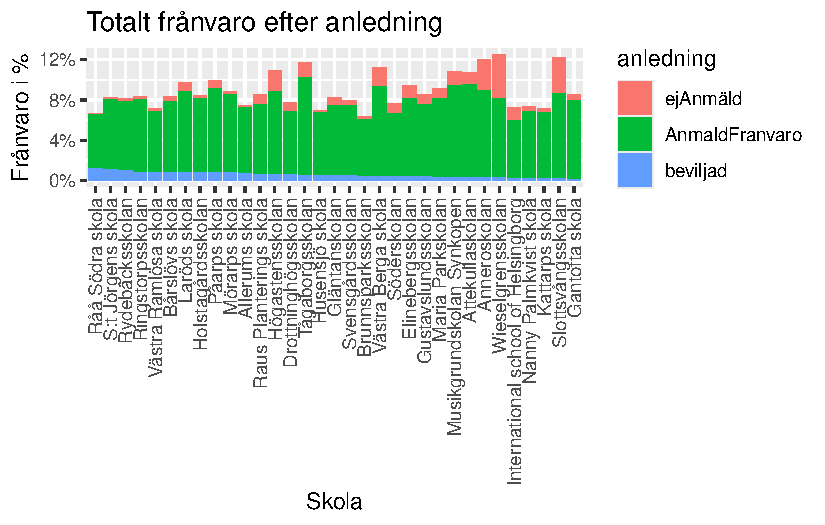
\includegraphics{test2_files/figure-pdf/unnamed-chunk-2-1.pdf}

\textbf{Vilka veckor är eleverna lediga som går på de skolor med högst
andel föräldrar med eftergymnasial utbildning?}
\includegraphics{Veckor 5 högsta utbildning.png} Vi noterar att det är
högre andel ledighet före- och efter lov. Exempelvis höstlovet v.44,
jullovet och sista veckan innan sommarlovet.

\textbf{Vilka veckor är eleverna lediga som går på de skolor med lägst
andel föräldrar med eftergymnasial utbildning?}
\includegraphics{Veckor 5 lägsta.png} Veckor som sticker ut är
exempelvis vecka 15 då ramadan avslutades och Eid al-Fitr inträffade,
samt veckan innan sommarlovet. Överlag är det dock sparsamt med beviljad
ledighet. Skillnaden känns iofs rimlig i att kapitalstarka hushåll har
större möjligheter att ta ledigt.

Den andra grafen visar också hur omfattande den oanmälda frånvaron är på
skolor i områden med socioekonomiska utmaningar.

\textbf{Den naturliga följdfrågan blir om den anmälda/oanmälda frånvaron
på dessa skolor kan vara föräldrastödd frånvaro, där exempelvis eleverna
är bortresta}

\begin{figure}

\centering{

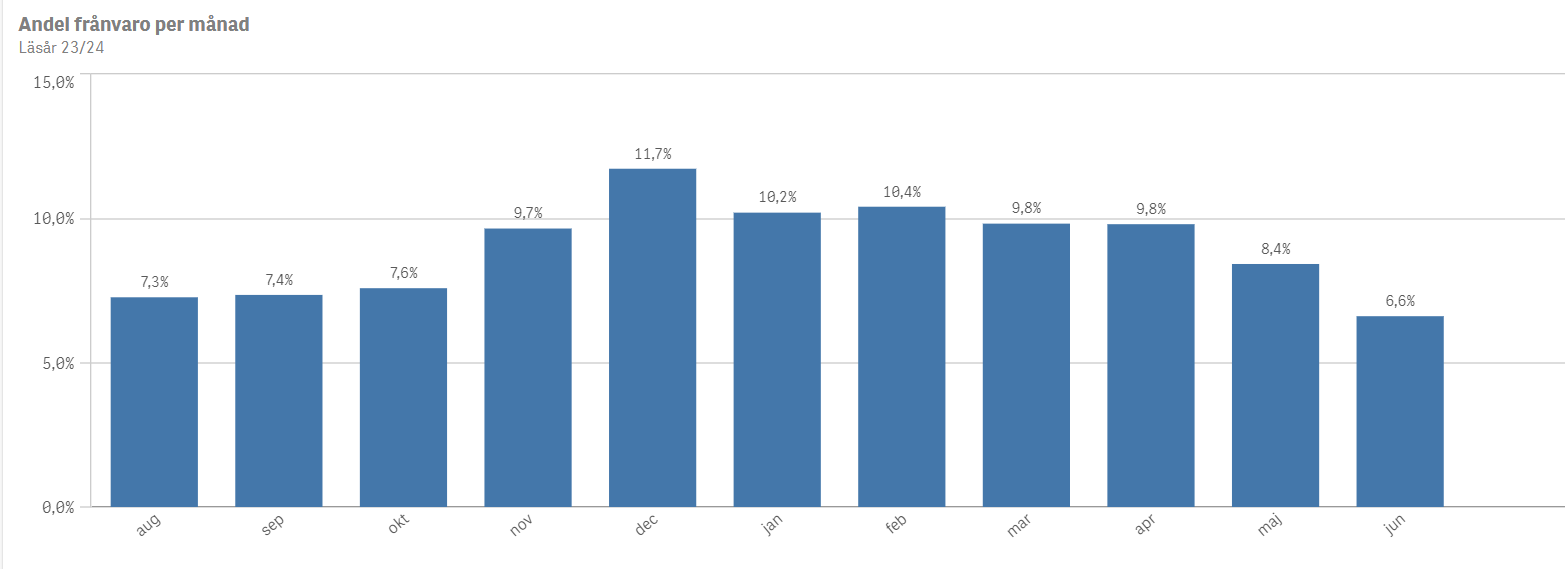
\includegraphics{monthj.png}

}

\caption{\label{fig-month}Frånvaro uppdelat efter månad}

\end{figure}%

Frånvaron vid våra skolor, uppdelad per månad, visar att augusti,
september och oktober har liknande nivåer av frånvaro, som illustrerat i
Figure~\ref{fig-month}. Detta mönster ger en utgångspunkt för att
undersöka om frånvaron är högre på vissa skolor i augusti jämfört med de
följande månaderna. En sådan skillnad kan potentiellt vara en indikator
på föräldrastödd frånvaro.

\begin{longtable}[t]{lrrr}
\caption{\label{tab:unnamed-chunk-3}Frånvaro per skola: Augusti jämfört med genomsnitt för september och oktober}\\
\toprule
Skola & Augusti & Medel sep/okt & Skillnad\\
\midrule
Wieselgrensskolan & 12.6 & 11.3 & 1.3\\
Västra Berga skola & 9.6 & 8.1 & 1.5\\
Raus Planterings skola & 9.1 & 6.7 & 2.4\\
Anneroskolan & 12.4 & 9.3 & 3.1\\
Drottninghögsskolan & 10.8 & 6.4 & 4.5\\
\bottomrule
\end{longtable}

I tabellen har jag identifierat fem skolor där det finns markanta
skillnader i frånvaron mellan augusti och de efterföljande månaderna,
exempelvis skiljer sig frånvaron i augusti och septembert/oktober hela
4,5 \%-enheter på Drottninghögskolan. Detta skulle kunna tyda på
föräldrastödd frånvaro. Men när vi analyserar vilka veckor eleverna
faktiskt är frånvarande, visar det sig att det inte är den första veckan
på höstterminen som sticker ut mest. Istället är det främst den tredje
och fjärde veckan som har högst frånvaro. Förlängda lov borde rimligtvis
påverka de första veckorna mest, och även om frånvaron är något högre då
jämfört med senare veckor i september och oktober, tyder
veckofördelningen ändå på att andra faktorer också spelar in.

\begin{figure}[H]

{\centering 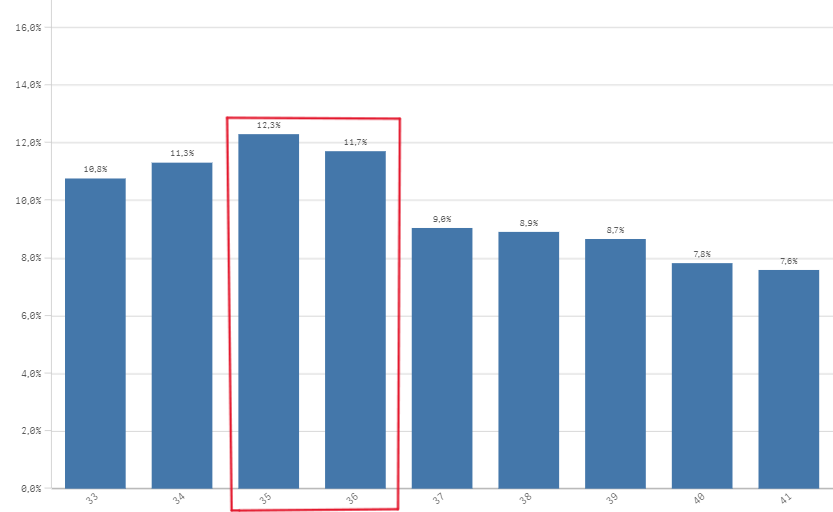
\includegraphics{firstweeks.png}

}

\caption{Första veckorna av höstterminen}

\end{figure}%

\textbf{Elevomsättning}

För många skolor så är det ingen omfattande förändring av elevgruppen de
första veckorna. Men lite analys av Wieselgrenskolan visar att HT23 så
försvann ca 20 elever de första 3-4 veckorna. Om vi tittar närmare på
deras data i frånvarostatistiken och Edlevo så framgår det att flertalet
av dessa elever aldrig dök upp till skolan eller flyttade men fortsatte
att registrera frånvaro. De hade således väldigt hög frånvaro men
försvann ur systemet efter ett par veckor. Att skolan hade ett 10-15
extra med nästan 100\% frånvaro kommer göra stor skillnad i
frånvarostatistiken (grovt uppskattat en 1-3 procentenheter).

\textbf{Är den ökade frånvaron i augusti på dessa skolor en indikation
på ett förlängt lov?}

Svårt att dra några slutsatser, det är onekligen en noterbar skillnad.
Däremot blir det väldigt tydligt av att ha undersökt siffrorna att
skolor med större förändringar i elevgruppen påverkar
frånvarostatistiken, speciellt för elever som inte dyker upp alls.



\end{document}
